\documentclass[letterpaper,11pt]{article}

% Soporte para los acentos.
\usepackage[utf8]{inputenc}
\usepackage[T1]{fontenc}
% Idioma español.
\usepackage[spanish,mexico, es-tabla]{babel}
% Soporte de símbolos adicionales (matemáticas)
\usepackage{multirow}
\usepackage{amsmath}
\usepackage{amssymb}
\usepackage{amsthm}
\usepackage{amsfonts}
\usepackage{mathtools}
\usepackage{latexsym}
\usepackage{enumerate}
\usepackage{ragged2e}
\usepackage{listings}
\usepackage{xcolor}
\usepackage{graphicx}
\usepackage{hyperref}
% Modificamos los márgenes del documento.                                       %
\usepackage[lmargin=2cm,rmargin=2cm,top=2cm,bottom=2cm]{geometry}

\definecolor{codegreen}{rgb}{0,0.6,0}
\definecolor{codegray}{rgb}{0.5,0.5,0.5}
\definecolor{codepurple}{rgb}{0.58,0,0.82}
\definecolor{backcolour}{rgb}{0.95,0.95,0.92}

\lstdefinestyle{mystyle}{
    backgroundcolor=\color{backcolour},   
    commentstyle=\color{codegreen},
    keywordstyle=\color{magenta},
    numberstyle=\tiny\color{codegray},
    stringstyle=\color{codepurple},
    basicstyle=\ttfamily\footnotesize,
    breakatwhitespace=false,         
    breaklines=true,                 
    captionpos=b,                    
    keepspaces=true,                 
    numbers=left,                    
    numbersep=5pt,                  
    showspaces=false,                
    showstringspaces=false,
    showtabs=false,                  
    tabsize=2
}

\lstset{style=mystyle}

\title{Facultad de Ciencias, UNAM \\ Redes Neuronales \\ Tarea 2}
\author{Rubí Rojas Tania Michelle}
\date{13 de abril de 202}

\begin{document}
\maketitle

\begin{enumerate}
    % Ejercicio 1.
    \item Usando \textit{sklearn.datasets.make\_moons} genera un conjunto de 
    datos de la siguiente forma:
    \begin{verbatim}
        In [1]: C1, C2 = moons(random state=123, n samples=200, noise=0.1)
    \end{verbatim}

    \begin{lstlisting}[language=Python]
    from sklearn.datasets import make_moons
    import matplotlib.pyplot as plt

    C1, C2 = make_moons(random_state = 123, n_samples=200, noise=0.1)
    plt.scatter(C1[:,0], C1[:,1], c = C2)
    plt.show()
    \end{lstlisting}

    \begin{figure}[ht]
        \centering
        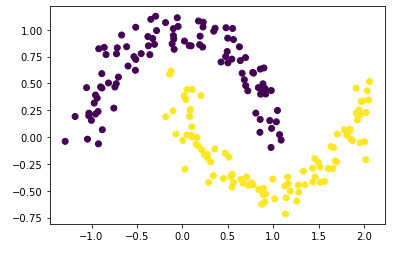
\includegraphics[width=0.45\textwidth]{./imagenes/datos.png}
    \end{figure}            

    \begin{enumerate}
        % Ejercicio 1.a
        \item Implementa la regresión logística usando el descenso gradiente 
        para clasificar $C_1$ y $C_2$.
        
        \textsc{Solución:}
        \begin{lstlisting}[language=Python]
        import numpy as np

        '''
        La funcion sigmoide es de la forma S(z) = 1/(1 + e^{-z}), donde 
        z = x * w^{T} + b. 
        '''
        def sigmoide(z):
            return 1 / (1 + np.exp(-z))

        def de_coste(y, y_hat):
            j = - (y.dot(np.log(y_hat)) + (1 - y).dot((np.log(1 - y_hat))))
            return j

        def descenso_gradiente(x, y, alpha, theta, num_iteraciones):
            costos = []
            for each_iter in range (num_iteraciones):
                z = np.dot(x, theta[1:]) + theta[0]
                y_hat = sigmoide(z)
                error = y_hat - y
                gradiente = x.T.dot(error)
                theta[0] -= alpha * error.sum()
                theta[1:] -= alpha * gradiente
                costos.append((1 / num_iteraciones) * (de_coste(y, y_hat)))
            return costos

        def prediccion(data):
            z = np.dot(data, theta[1:]) + theta[0]
            return np.where(sigmoide(z)>= 0.5, 0, 1)
        \end{lstlisting}

        Asignando valores a $\theta$, $\alpha$ y al número de iteraciones, 
        obtenemos
        \begin{lstlisting}[language=Python]
        k, l = C1.shape
        theta = np.zeros(l+1)
        costo = descenso_gradiente(C1, C2, 0.0001, theta, 10000)

        print ('Interseccion:', theta[0])
        print ('Coeficientes estimados:', theta[1:])

        # Visualizamos la funcion de costo.
        plt.title('Funcion de Costo J')
        plt.xlabel('Numero de iteraciones')
        plt.ylabel('Costo')
        plt.plot(costo)
        plt.show()
        \end{lstlisting}

        \begin{verbatim}
        Intersección: 0.5894707477910425
        Coeficientes estimados: [ 1.15656526 -4.85276922]
        \end{verbatim}

        \begin{figure}[ht]
            \centering
            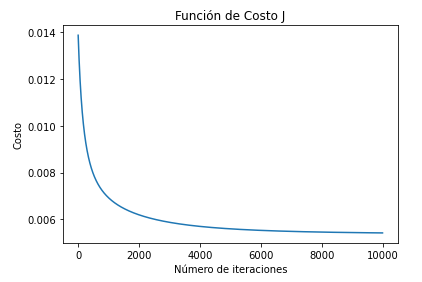
\includegraphics[width=0.6\textwidth]{./imagenes/costo.png}
            \label{coste}
        \end{figure}  

        \newpage
        Finalmente, la clasificación quedaría de la siguiente forma:
        \begin{lstlisting}[language=Python]
        plt.scatter(C1[:,0], C1[:,1], c = prediccion(C1))
        plt.show()
        \end{lstlisting}

        \begin{figure}[ht]
            \centering
            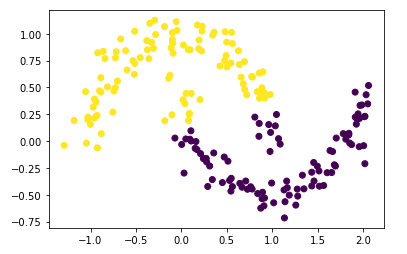
\includegraphics[width=0.55\textwidth]{./imagenes/clasificacion.png}
        \end{figure} 

        Utilizando \textbf{sklearn} para comprar los resultados obtenemos
        \begin{lstlisting}[language=Python]
        from sklearn.linear_model import LogisticRegression

        regresion_logistica = LogisticRegression()
        modelo = regresion_logistica.fit(C1, C2)

        print ("Interseccion: ", modelo.intercept_)
        print ("Coeficientes estimados: ", modelo.coef_)

        # Visualizamos la clasificacion.
        plt.scatter(C1[:,0], C1[:,1], c = regresion_logistica.predict(C1))
        plt.show()
        \end{lstlisting}

        \begin{verbatim}
        Intersección:  [0.36023346]
        Coeficientes estimados:  [[ 1.09045248 -3.69780292]]
        \end{verbatim}

        \begin{figure}[h]
            \centering
            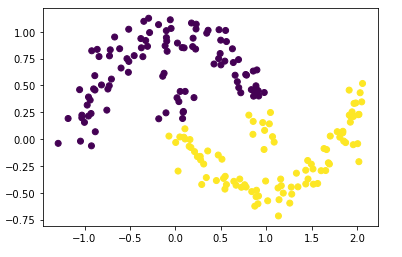
\includegraphics[width=0.55\textwidth]{./imagenes/revision.png}
        \end{figure} 

        % Ejercicio 1.b
        \item ¿Qué transformación de los datos ocupaste para poder hacer la
        correcta clasificación?

        \textsc{Solución:} Sabemos que la función \textit{sigmoide} 
        \begin{equation*}
            S(z) = \frac{1}{1 + e^{-z}} \; \; \; \; \; \; \; \; \; \; \; \; \;
            z = w^{T} x + b
        \end{equation*}
        
        nunca llega a tocar el eje de las $y$ a $0$ o $1$, y se mueve entre 
        estos dos valores. 
        \begin{figure}[h]
            \centering
            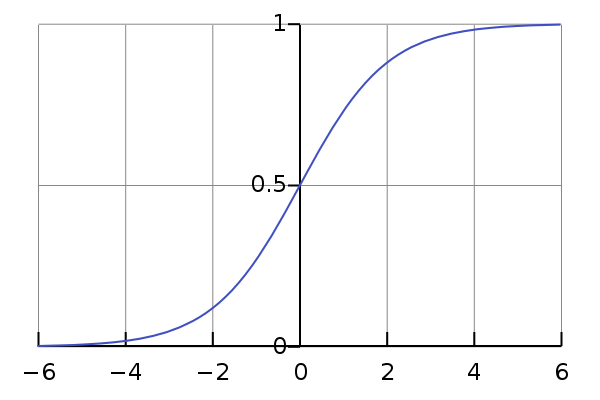
\includegraphics[width=0.4\textwidth]{./imagenes/sigmoide.png}
        \end{figure} 
        
        Lo cual la hace perfecta para expresar una propabilidad para nuestra 
        decisión binaria (clasificar).

        Ahora bien, debemos encontrar los valores correctos de $w$ y $b$ que 
        nos permitan encontrar el valor correcto de la función $S$. El vector 
        de pesos $w$ se inicializa de manera arbitraria (aunque en nuestra 
        implementación lo inicializamos como el vector cero). 

        Para saber qué tan bien o qué tan mal logra clasificar nuestra función,
        requerimos una función de error o de coste. Y teniéndo en cuenta que 
        nuestro problema no es convexo, entonces sería de la forma 
        \begin{equation*}
            L(y', y) = - (y \log y' + (1 - y) \log (1 - y'))
        \end{equation*}

        Esta función únicamente se usará sobre una entrada del conjunto de 
        datos. Ahora, para obtener una imagen general sobre el error de los 
        parámetros con respecto al total de los datos, usaremos la función de 
        costo, que es definida como:
        \begin{align*}
            J(w, b) 
            &= \frac{1}{m} \sum_{i=1}^{m} L(y'^i, y^i) \\ 
            &= - \frac{1}{m} \sum_{i=1}^{m} [y^i \log y'^i + 
               (1 - y^i) \log (1 - y'^i)]
        \end{align*}

        El objetivo es minimizar el costo total del modelo, para así acercarnos
        lo más posible a nuestras clases dadas $y$. Esta minimización la 
        hacemos utilizando el \textit{descenso gradiente}. 

        Por lo tanto, la función \textit{sigmoide} usa los datos de entrada y 
        los valores del modelo $\theta$ para minimizar la función de coste con 
        ayuda del algoritmo del desceso. Ésta es la transformación de los 
        datos que se va realizando, y se puede ver en la gráfica de 
        función de coste \ref{coste} . 
    \end{enumerate}

    \newpage
    % Ejercicio 2.
    \item Calcula la derivada de la tangente hiperbólica $\tanh$.
    
    \textsc{Solución:}
    \begin{align*}
        \frac{d}{dx} \tanh (x) 
        &= \frac{d}{dx} \left(\frac{\sinh (x)}{\cosh (x)}\right)
        && \text{definición de $\tanh (x)$} \\
        &= \frac{(\sinh' (x) \cdot \cosh (x)) - (\cosh' (x) \cdot \sinh (x))}
                {\cosh^2 (x)}
        && \text{derivative quotient rule} \\ 
        &= \frac{(\cosh (x) \cdot \cosh (x)) - (\sinh (x) \cdot \sinh (x))}
                {\cosh^2 (x)}
        && \text{$\sinh' (x) = \cosh (x)$ y $\cosh' (x) = \sinh (x)$} \\ 
        &= \frac{\cosh^2 (x) - \sinh^2 (x)}{\cosh^2 (x)}
        && \text{aritmética} \\ 
        &= \frac{1}{\cosh^2 (x)}
        && \text{$\cosh^2 (x) - \sinh^2 (x) = 1$} \\ 
        &= sech^2 (x)
        && \text{$\frac{1}{\cosh^2} = sech^2 (x)$}
    \end{align*}

    % Ejercicio 3.
    \item Usando el perceptrón multicapa visto en clase, clasifica a $C_1$ y 
    $C_2$. ¿Qué parámetros ocupaste?

    \textsc{Solución:} Primero, generamos un conjunto de datos. 
    \begin{lstlisting}[language=Python]
    from sklearn.datasets import make_moons
    import matplotlib.pyplot as plt

    C1, C2 = make_moons(random_state = 123, n_samples=200, noise=0.1)
    plt.scatter(C1[:,0], C1[:,1], c = C2)
    plt.show()
    \end{lstlisting}

    \begin{figure}[ht]
        \centering
        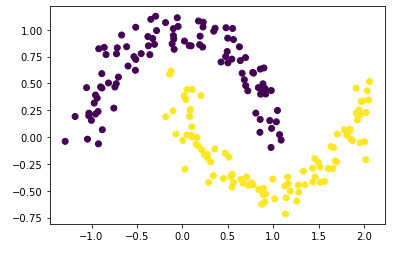
\includegraphics[width=0.45\textwidth]{./imagenes/datos.png}
    \end{figure}  
    
    Apoyándonos del \textbf{MLPClassifier} para clasificar el conjunto de 
    datos, obtenemos 
    \begin{lstlisting}[language=Python]
    from sklearn.neural_network import MLPClassifier
    from sklearn.model_selection  import train_test_split                       
    import matplotlib.pyplot as plt

    # Dividimos al conjunto de datos para poder manejarlo.
    X_train, X_test, y_train, y_test = train_test_split(C1, C2)

    # Aqui podemos observar los parametros que utilizamos.
    modelo = MLPClassifier(activation = 'tanh', max_iter = 1000, 
                           learning_rate_init = 0.001, hidden_layer_sizes = (10,4))

    modelo.fit(X_train, y_train)


    # Visualizamos la clasificacion con los datos de prueba. 
    plt.scatter(X_test[:,0], X_test[:,1], c = modelo.predict(X_test))
    plt.show()

    fig = plt.figure()
    ax1 = fig.add_subplot(111)
    # Visualizamos la clasificacion con los datos de prueba y entrenamiento.
    ax1.scatter(X_test[:,0], X_test[:,1], c = modelo.predict(X_test))
    ax1.scatter(X_train[:,0], X_train[:,1], c = modelo.predict(X_train))
    plt.show()
    \end{lstlisting}

    \begin{figure}[ht]
        \centering
        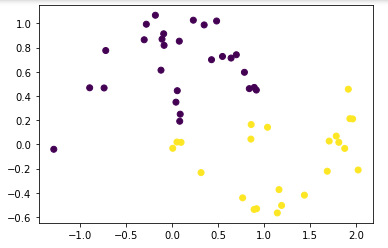
\includegraphics[width=0.4\textwidth]{./imagenes/clasificacion2-1.png}
    \end{figure} 

    \begin{figure}[ht]
        \centering
        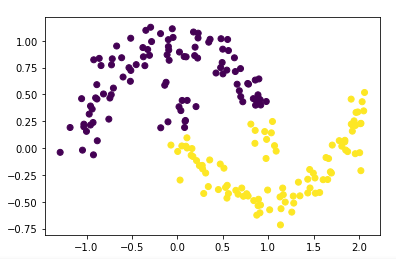
\includegraphics[width=0.4\textwidth]{./imagenes/clasificacion2-2.png}
    \end{figure} 

    % Ejercicio 4.
    \item Con la red neuronal, vista en clase, que hace la clasificación 
    multiclase usando la función \textit{softmax}, realiza los siguiente 
    ejercicios:
    \begin{enumerate}
        % Ejercicio 4.a
        \item Encuentra la mejor arquitectura para el conjunto de Iris. 
        Justifica tu respuesta de por qué es la mejor.

        \textsc{Solución:} Dado un vector de entrada, queremos poder clasificarlo
        en \textit{Setosa}, \textit{Versícolor} o \textit{Virginica}. 

        Tomando el siguiente esquema como referencia
        \begin{figure}[ht]
            \centering
            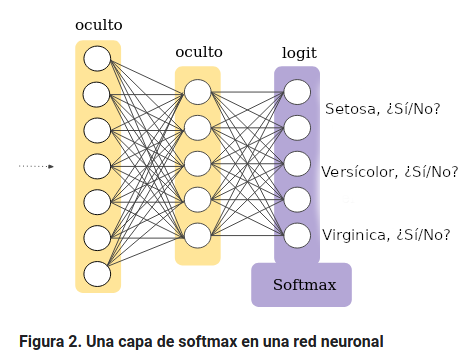
\includegraphics[width=0.31\textwidth]{./imagenes/softmax.png}
        \end{figure} 

        podemos visualizar un poco mejor la arquitectura elegida:
        \begin{itemize}
            \item Capa de entrada.
            Tendremos 4 neuronas, una por cada entrada de nuestro vector de 
            inicio. Cada uno de estos vectores se ve de la forma:
            \begin{equation*}
                v = [l \; \; a \; \; l \; \; a]
            \end{equation*}

            donde $l$ es el largo del sépalo y $a$ es el ancho del sépalo.
            
            \item Capa oculta.
            Tendremos ocho neuronas. Esta elección la hice basándome en una 
            implementación que encontré (donde utilizan softmax) para clasificar 
            la flor Iris. 
            
            Al principio probé con tres y cuatro neuronas en esta capa, pero no
            lograba que la tasa de aprendizaje y el número de iteraciones 
            lograran un buen resultado al momento de hacer las clasificaciones
            con los vectores de entrada (las entradas en el vector que regresa
            la función \textit{predict} eran muy parecidas entre sí, (casi 
            siempre un $0.33...$) y definitivamente esto no es lo que nosotros
            estamos buscando). Por lo que, esta arquitectura es la mejor para mí 
            (ya que funciona). 

            \item Capa de salida.
            Tendremos tres neuronas, una por cada especie relacionada a la flor
            Iris.
        \end{itemize}
        
        % Ejercicio 4.b
        \item Usa las funciones $\tan h$ y $\gamma$ en la capa intermedia. ¿Cuál
        funciona mejor?

        \textsc{Solución:} Primero, generamos el conjunto de datos \textbf{Iris}.
        \begin{lstlisting}[language=Python]
        from sklearn.datasets import load_iris
        import matplotlib.pyplot as plt 

        # Cargamos el conjunto de datos. 
        iris = load_iris()
        # Creamos la matriz de caracteristicas.
        X = iris.data
        # Creamos el vector de caracteristicas.
        y = iris.target

        # Visualizamos los puntos de entrenamiento.
        plt.scatter(X[:,0], X[:,1], c = y)
        plt.xlabel('Largo del sepalo')
        plt.ylabel('Ancho del sepalo')
        plt.show()
        \end{lstlisting}

        \begin{figure}[ht]
            \centering
            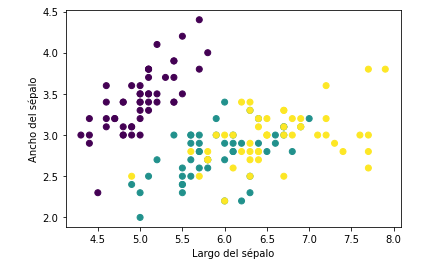
\includegraphics[width=0.5\textwidth]{./imagenes/iris.png}
        \end{figure}

        Los estímulos (vectores de entrada) son codificados para mostrar un $1$
        en entrada correspondiente a su valor, por ejemplo
        \begin{equation*}
            2 = [0, 0, 1]
        \end{equation*}

        \newpage
        \begin{lstlisting}[language=Python]
        from sklearn.preprocessing import OneHotEncoder

        y = iris.target.reshape(-1,1)
        encoder = OneHotEncoder(sparse=False)
        y = encoder.fit_transform(y)
        \end{lstlisting}

        Ahora, no sólo queremos un valor entre $0$ y $1$, sino que queremos un 
        vector en el que la salida deseada marque un $1$ y los demás $0$ (o 
        algo cercano, en ambos casos). Es decir, no podemos usar $n$ 
        \textit{sigmoides} porque el valor de cada entrada está condicionada a
        ser $1$ sólo si los demás dan $0$.

        Esto se puede lograr con la función \textit{Softmax} que nos da la 
        probabilidad $i$-ésima de cada entrada en el vector aleatorio $x$.
        \begin{equation*}
            p_i = \frac{e^{x_i}}{\sum_{j}^{N} e^{x_j}}
        \end{equation*}

        Pero ahora no podemos usar el $MSE$ (ni $MAE$) como nuestra función de 
        error. Debemos usar algo que nos permita ponderar el error de haberle
        \textit{atinado} a la entrada deseada con un $1$, y con un $0$ a las 
        demás.

        \textit{Cross-Entropy} es la función que generaliza a la función que 
        usamos para el caso binario.
        \begin{equation*}
            CE = \sum_{i}^{N} y_i \log (x_i)
        \end{equation*}

        El paso siguiente es definir los parámetros, la arquitectura (definida 
        en el inciso anterior) y las funciones que vamos a utilizar:
        \begin{lstlisting}[language=Python]
        import numpy as np

        def sigmoide(z):
            return 1 / (1 + np.exp(-z))

        def sigmoide_prima(x):
            return sigmoide(x) * (1 - sigmoide(x))

        def tanh(x):
            return ((np.exp(x) - np.exp(-x)) / (np.exp(x) + np.exp(-x)))

        def tanh_prima(x):
            return (1 / (np.exp(x) + np.exp(-x))**2)

        def softmax(A):
            expA = np.exp(A)
            return expA / expA.sum(axis = 1, keepdims = True)

        N = X.shape[0]  # numero de instancias
        n = X.shape[1]  # dimension de instancias
        nh =  3         # numero de neuronas ocultas
        m = 3           # dimension salida

        wh = np.random.rand(n,nh)  # pesos escondidos
        bh = np.random.randn(nh)   # nodo sesgo escondidos

        wo = np.random.rand(nh,m)  # pesos salida
        bo = np.random.randn(m)    # nodo salida
        lr = 0.00001               # tasa
        \end{lstlisting}

        \newpage
        Ahora, realizamos el entrenamiento usando la función $\tanh$
        \begin{lstlisting}[language=Python]
        from sklearn.model_selection import train_test_split

        # Dividimos nuestro conjunto de datos para poder manejarlo.
        Xt, Xs, yt, ys = train_test_split(X,y)

        J = []
        for epoca in range (5000):
            # Retropropagacion
            
            # Feed forward
            zh = np.dot(X_train, wh) + bh   # activacion escondidas
            ah = tanh(zh)                   # disparo escondidas

            zo = np.dot(ah, wo) + bo        # activacion salida 
            ao = softmax(zo)                # disparo salida (neuronas salida)
            
            # Envio de error hacia atras
            
            # Capa salida - escondida  
            error = ao - y_train

            deltas_wo = np.dot(ah.T, error)
            deltas_bo = error

            # Capa escondida - entrada
            temp_dah = np.dot(error , wo.T)
            deriv_h = tanh_prima(zh)

            deltas_wh = np.dot(X_train.T, deriv_h * temp_dah)
            deltas_bh = temp_dah * deriv_h

            # Actualizacion de pesos
            wh -= lr * deltas_wh
            bh -= lr * deltas_bh.sum(axis=0)

            wo -= lr * deltas_wo
            bo -= lr * deltas_bo.sum(axis=0)
            
            if epoca % 200 == 0:
                logL = np.sum(-y_train * np.log(ao))
                J.append(logL)
        \end{lstlisting}

        \begin{figure}[ht]
            \centering
            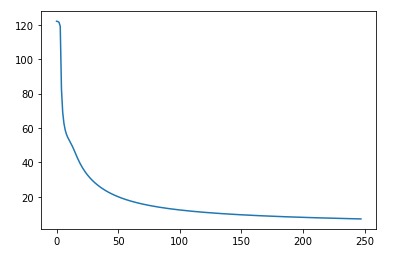
\includegraphics[width=0.35\textwidth]{./imagenes/logL-tan.png}
        \end{figure}

        Realizamos el entrenamiento también con la funcion $\gamma$.
        \begin{lstlisting}[language=Python]
        from sklearn.model_selection import train_test_split

        # Dividimos nuestro conjunto de datos para poder manejarlo.
        X_train, X_test, y_train, y_test = train_test_split(X, y)

        J = []
        for epoca in range (50000):
            # Retropropagacion
            
            # Feed forward
            zh = np.dot(X_train, wh) + bh   # activacion escondidas
            ah = sigmoide(zh)               # disparo escondidas
            zo = np.dot(ah, wo) + bo        # activacion salida 
            ao = softmax(zo)                # disparo salida
            
            # Envio de error hacia atras
            
            # Capa salida - escondida  
            error = ao - y_train

            deltas_wo = np.dot(ah.T, error)
            deltas_bo = error

            # Capa escondida - entrada
            temp_dah = np.dot(error , wo.T)
            deriv_h = sigmoide_prima(zh)

            deltas_wh = np.dot(X_train.T, deriv_h * temp_dah)
            deltas_bh = temp_dah * deriv_h

            # Actualizacion de pesos
            wh -= lr * deltas_wh
            bh -= lr * deltas_bh.sum(axis=0)

            wo -= lr * deltas_wo
            bo -= lr * deltas_bo.sum(axis=0)
            
            if epoca % 200 == 0:
                logL = np.sum(-y_train * np.log(ao))
                print('logL function value: ', logL)
                J.append(logL)

        plt.plot(J[2:])
        \end{lstlisting}

        \begin{figure}[ht]
            \centering
            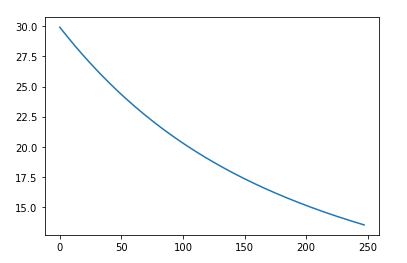
\includegraphics[width=0.5\textwidth]{./imagenes/logL-sig.png}
        \end{figure}

        % Ejercicio 4.c
        \item Clasifica los siguientes estímulos y reporta a qué clase pertenece
        cada uno:
        \begin{itemize}
            \item $5.97 \; 4.20 \; 1.23 \; 0.25$
            \item $6.80 \; 5.00 \; 1.25 \; 1.20$
            \item $12.50 \; 9.20 \; 40.32 \; 21.55$
        \end{itemize}

        \textsc{Solución:} Utlizamos la función 
        \begin{lstlisting}[language=Python]
        def predict(wh, wo, fact1, fact2, x):
            zh = np.dot(x.T, wh) + bh           # activacion escondidas
            ah = fact1(zh)                      # disparo escondidas
            
            zo = np.dot(ah, wo) + bo            # activacion salida 
            ao = fact2(zo)                      # disparo salida
            return ao
        \end{lstlisting}

        para clasificar los estímulos solicitados:
        \begin{itemize}
            \item Con la función de activación $\tanh$.
            \begin{lstlisting}[language=Python]
                d
            \end{lstlisting}

            Por lo tanto, los dos primeros vectores corresponden a la especie 
            \textit{setosa} y el último corresponde a la especie 
            \textit{virginica}.

            \item Con la función de activacion $\gamma$.
            \begin{lstlisting}[language=Python]
            v1 = np.array([[5.97],[4.20],[1.23],[0.25]])
            v2 = np.array([[6.80],[5.00],[1.25],[1.20]])
            v3 = np.array([[12.50],[9.20],[40.32],[21.55]])

            p1 = predict(wh, wo, sigmoide, softmax, v1)
            p2 = predict(wh, wo, sigmoide, softmax, v2)
            p3 = predict(wh, wo, sigmoide, softmax, v3)

            print(p1)
            print(p2)
            print(p3)
            \end{lstlisting}

            \begin{verbatim}
                [[0.96800806 0.02926022 0.00273171]]
                [[0.96823689 0.02905003 0.00271307]]
                [[0.00214928 0.03275745 0.96509327]]
            \end{verbatim}

            Por lo tanto, los dos primeros vectores corresponden a la especie 
            \textit{setosa} y el último corresponde a la especie 
            \textit{virginica}.
        \end{itemize}

        % Ejercicio 4.d
        \item ¿Te parecen correctas todas las clasificaciones? En caso de que 
        alguna no, ¿por qué? ¿cómo corregirías este error?

        \textsc{Solución:} 
    \end{enumerate}

    % Ejercicio 5.
    \item ¿Qué es y cómo funciona la función de activación \textit{Radial Basis
    Function (RBF)}?

    \textsc{Solución:} Una \textit{función de base radial} $\phi(x)$ es una 
    función que calcula la distancia euclideana de un vector de entrada $x$
    respecto de un centro $c$, de tal manera que resulta la siguiente función:
    \begin{equation*}
        f(x) = (\| x - c_i\|)
    \end{equation*}

    A cada neurona de la capa de entrada le corresponde una función de base 
    radial $\Phi (x)$ y un peso de salida $w_i$. El patrón de salida ingresa a
    una neurona de salida que suma las entradas y da como resultado una salida.
    La función de una red $RBF$ final resulta:
    \begin{equation*}
        F(x) = \sum^N_{i=1} w_{i} \Phi (\| x - c_{i} \|)
    \end{equation*} 

    Las redes $RBF$ tienen una construcción rígida de tres capas:
    \begin{figure}[ht]
        \centering
        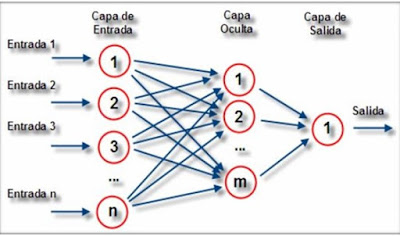
\includegraphics[width=0.4\textwidth]{./imagenes/rbf.png}
    \end{figure}  

    \begin{itemize}
        \item \textbf{Capa de Entrada}. Transmiten las señales de entrada a las 
        neuronas ocultas sin realizar procesamiento, es decir, las conexiones de 
        la capa de entrada a la capa oculta no llevan pesos asociados. 

        \item \textbf{Capa Oculta}. Realizan una transformación local y no lineal 
        de dichas señales.

        Cada elemento de procesado $i$ de la capa oculta tiene asociada una 
        función de base radial de tal manera que representa una clase o 
        categoría, donde dicha clase viene dada por $(C_i, d_i)$. $C_i$
        representa un centro de cluster (pesos asociados a cada neurona $i$) y 
        $d_i$ representa la desviación, anchura o dilatación de la función de 
        base radial asociada a dicho elemento. 

        La salida de cada elemento de la capa oculta $z_i (n)$ se calcula como 
        ls distancia que existe entre el patrón de entrada $X (n)$ al centro del 
        clouster $C_i$ ponderada inversamente por $d_i$, y aplicando después a 
        ese valor una función de base radial.
        \begin{equation*}
            z_i (n) = 
            \Phi \left(\frac{\left( \sum^p_{j=1} \left( x_j (n) - c_{ji} 
                                                 \right)^2 \right)^{\frac{1}{2}}}
                            {d_i} \right) \; \; \; \; \; \; \; \; \; 
            i \in \{1, 2, ..., m\}
        \end{equation*}

        donde $\Phi$ es una función de base radial, dentro de éstas la más 
        utilizada es la función Gaussiana 
        \begin{equation*}
            \Phi (r) = e^{\frac{-r^2}{2}}
        \end{equation*}

        \item \textbf{Capa de Salida}. Realiza una combinación de las actividades 
        de las neuronas ocultas. Tiene la responsabilidad en la red de activación 
        de patrones aplicados en la capa de entrada. 

        Cada elemento de procesado calcula su valor neto como una combinación
        lineal de las salidas de los elementos de procesado de la capa oculta.
        La función de activación y transferencia es lineal, por lo que para un 
        patrón $n$, $X(n) = (x_1 (n), x_2 (n), ..., x_p (n))$, la salida de la 
        red asociada a cada elemento $k$ de la capa de salida se obtiene de la 
        forma 
        \begin{equation*}
            y_k (n) = \sum^m_{i=1} w_{ik} z_i (n) + \mu_k \; \; \; \; \; \; \;
            k \in \{1, 2, ..., r\}
        \end{equation*}

        donde los $w_{ik}$ son los pesos asociados al elemento $k$ de la capa 
        oculta y el elemento $i$ de la capa oculta, que ponderan cada uno las 
        salidas $z_i (n)$ del elemento de procesado de la capa oculta 
        correspondiente. 

        El término $\mu_k$ es un término denominado umbral y está asociado a
        cada uno de los elementos de procesado de la capa de salida. 
    \end{itemize}

    El aprendizaje consiste en la determinación de centros, desviaciones y pesos 
    de la capa oculta a la capa de salida. Como las capas de la red realizan 
    diferentes tareas, se separaán los parámetros de la capa oculta de la capa 
    de salida para optimizar el proceso. De esta forma, los centros y las 
    desviaciones siguen un proceso guiado por una optimización en el espacio de 
    entrada, mientras que los pesos siguen una optimización sobre la base de las 
    salidas que se desean obtener. 

    Los métodos de aprendizaje más utilizados son el \textit{método híbrido} y
    el \textit{método totalmente supervisado}. 
\end{enumerate}

\textbf{Bibliografía}
\begin{itemize}
    \item \url{https://medium.com/@dtellogaete/regresi%C3%B3n-log%C3%ADstica-en-
               python-y-r-machine-learning-02-fa066b3add09}
    \item \url{http://www.eenube.com/index.php/ldp/machine-learning/121-
               programar-una-red-neuronal-para-clasificacion-binaria}
    \item \url{https://www.interactivechaos.com/manual/tutorial-de-machine-
               learning/perceptron-multicapa}
    \item \url{https://analisisydecision.es/machine-learnig-analisis-grafico-
               del-funcionamiento-de-algunos-algoritmos-de-clasificacion/}
    \item \url{https://www.analyticslane.com/2020/04/20/entrenamiento-validacion-
               y-test-con-scikit-learn/}
    \item \url{https://chrisalbon.com/machine_learning/basics/loading_scikit-
               learns_iris_dataset/}
    \item \url{https://scikit-learn.org/stable/modules/generated/sklearn.datasets.
               load_iris.html}
    \item \url{https://developers.google.com/machine-learning/crash-course/multi-
               class-neural-networks/softmax?hl=es-419}
    \item \url{https://blog.crespo.org.ve/2018/02/}
    \item \url{https://www.wikiwand.com/es/RNA_de_base_radial#/Referencias}
    \item \url{http://ele.aut.ac.ir/~abdollahi/Lec_3_NN11.pdf}
    \item \url{http://dianainteligenciaartificial.blogspot.com/2015/07/redes-de-
               neuronas-de-base-radial.html}
    \item \url{http://www.varpa.org/~mgpenedo/cursos/scx/archivospdf/Tema5-6.pdf}
\end{itemize}
\end{document}
